\chapter{Results}
\label{chapter:appendix_results}
%%%%%%%%%%%%%%%%%%%%%%%%%%%%%%%%%%%%%%%%%%%%%%%%%%%%%%%%%%%%%%%%%%%%%%%%%%%%%%%%%%%%%

This is to present appendix chapters.

\begin{figure}[p]
    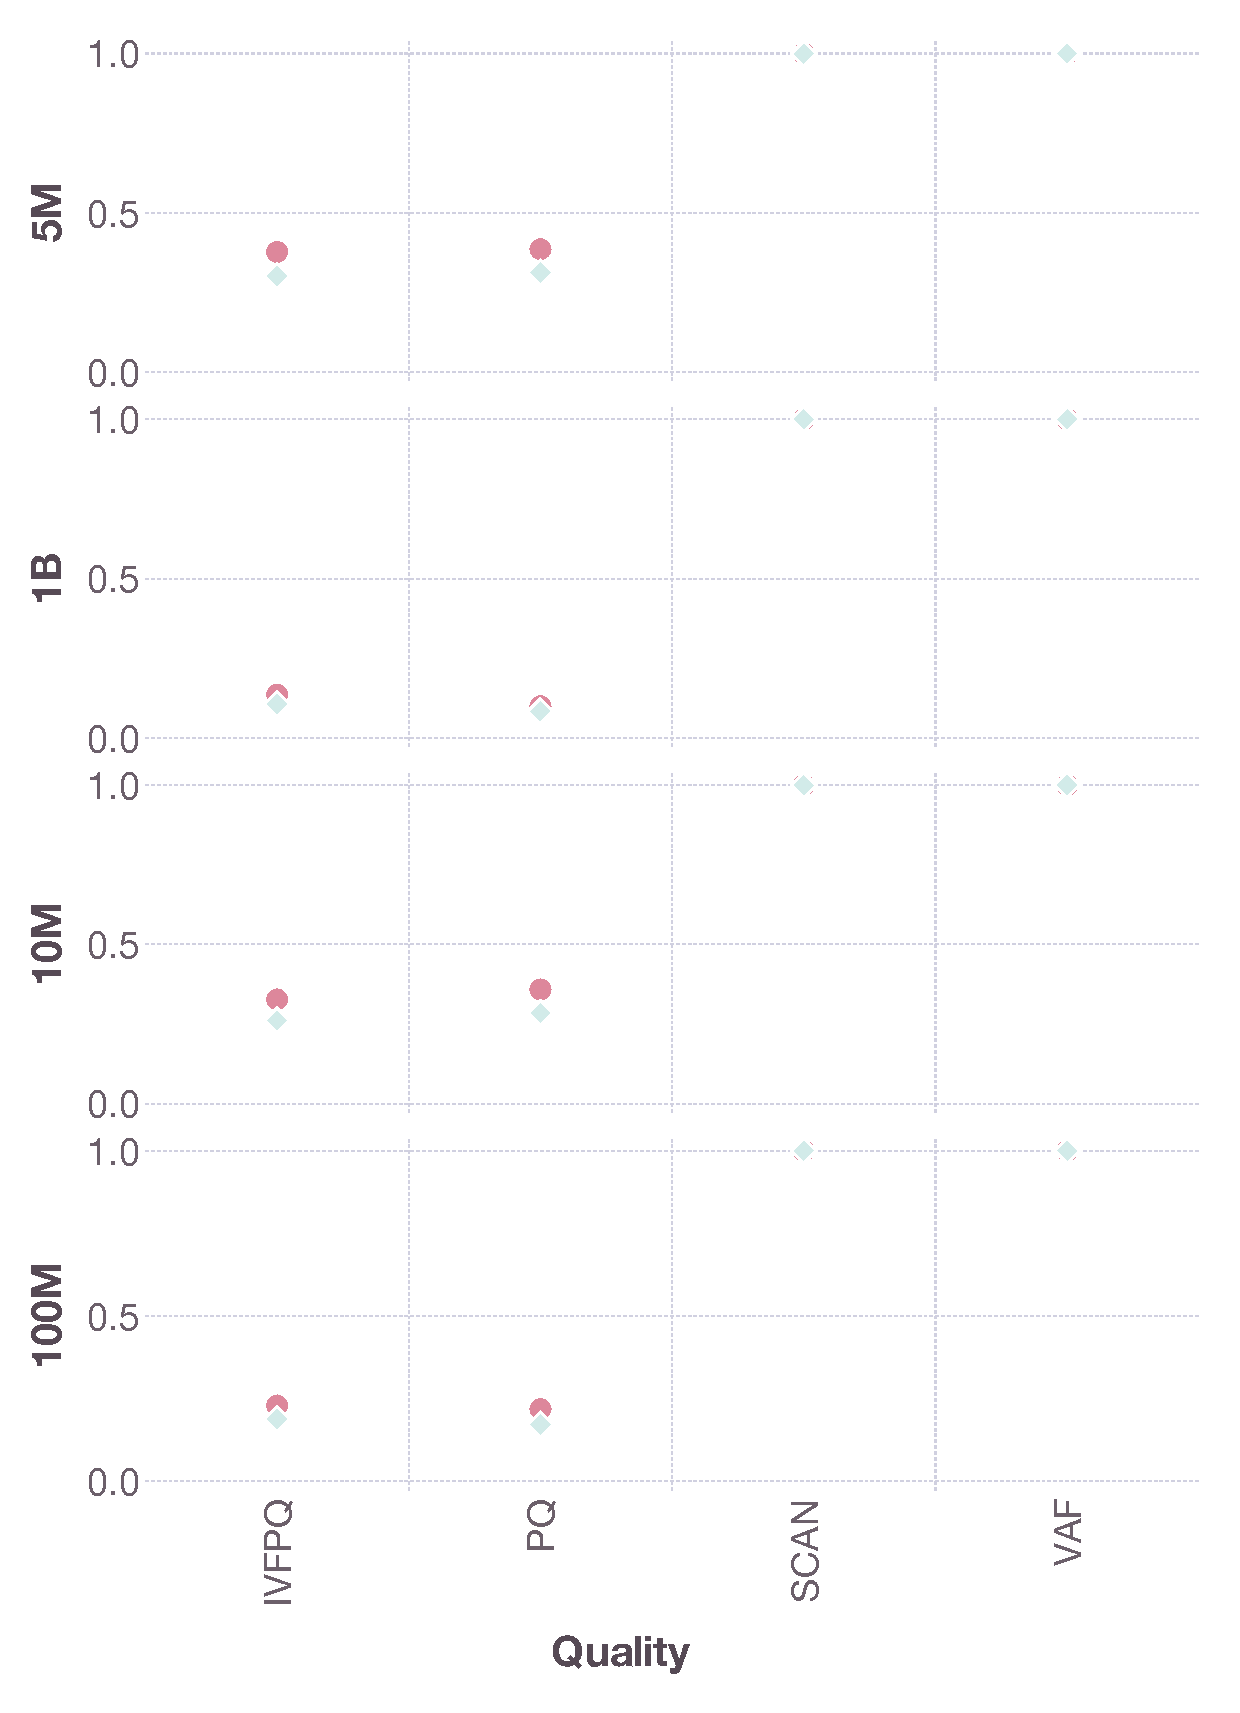
\includegraphics[width=\linewidth]{figures/bignns-cottontail-NNS-quality}
    \caption{Quality metrics for Cottontail DB during the simple \acrshort{nns} large-scale retrieval evaluation presented in \Cref{section:evaluation_bignns_cottontail}. Recall and \acrshort{dcg} are 1.0 for all execution strategies other than \acrshort{pq}.}
\end{figure}

\begin{figure}[p]
    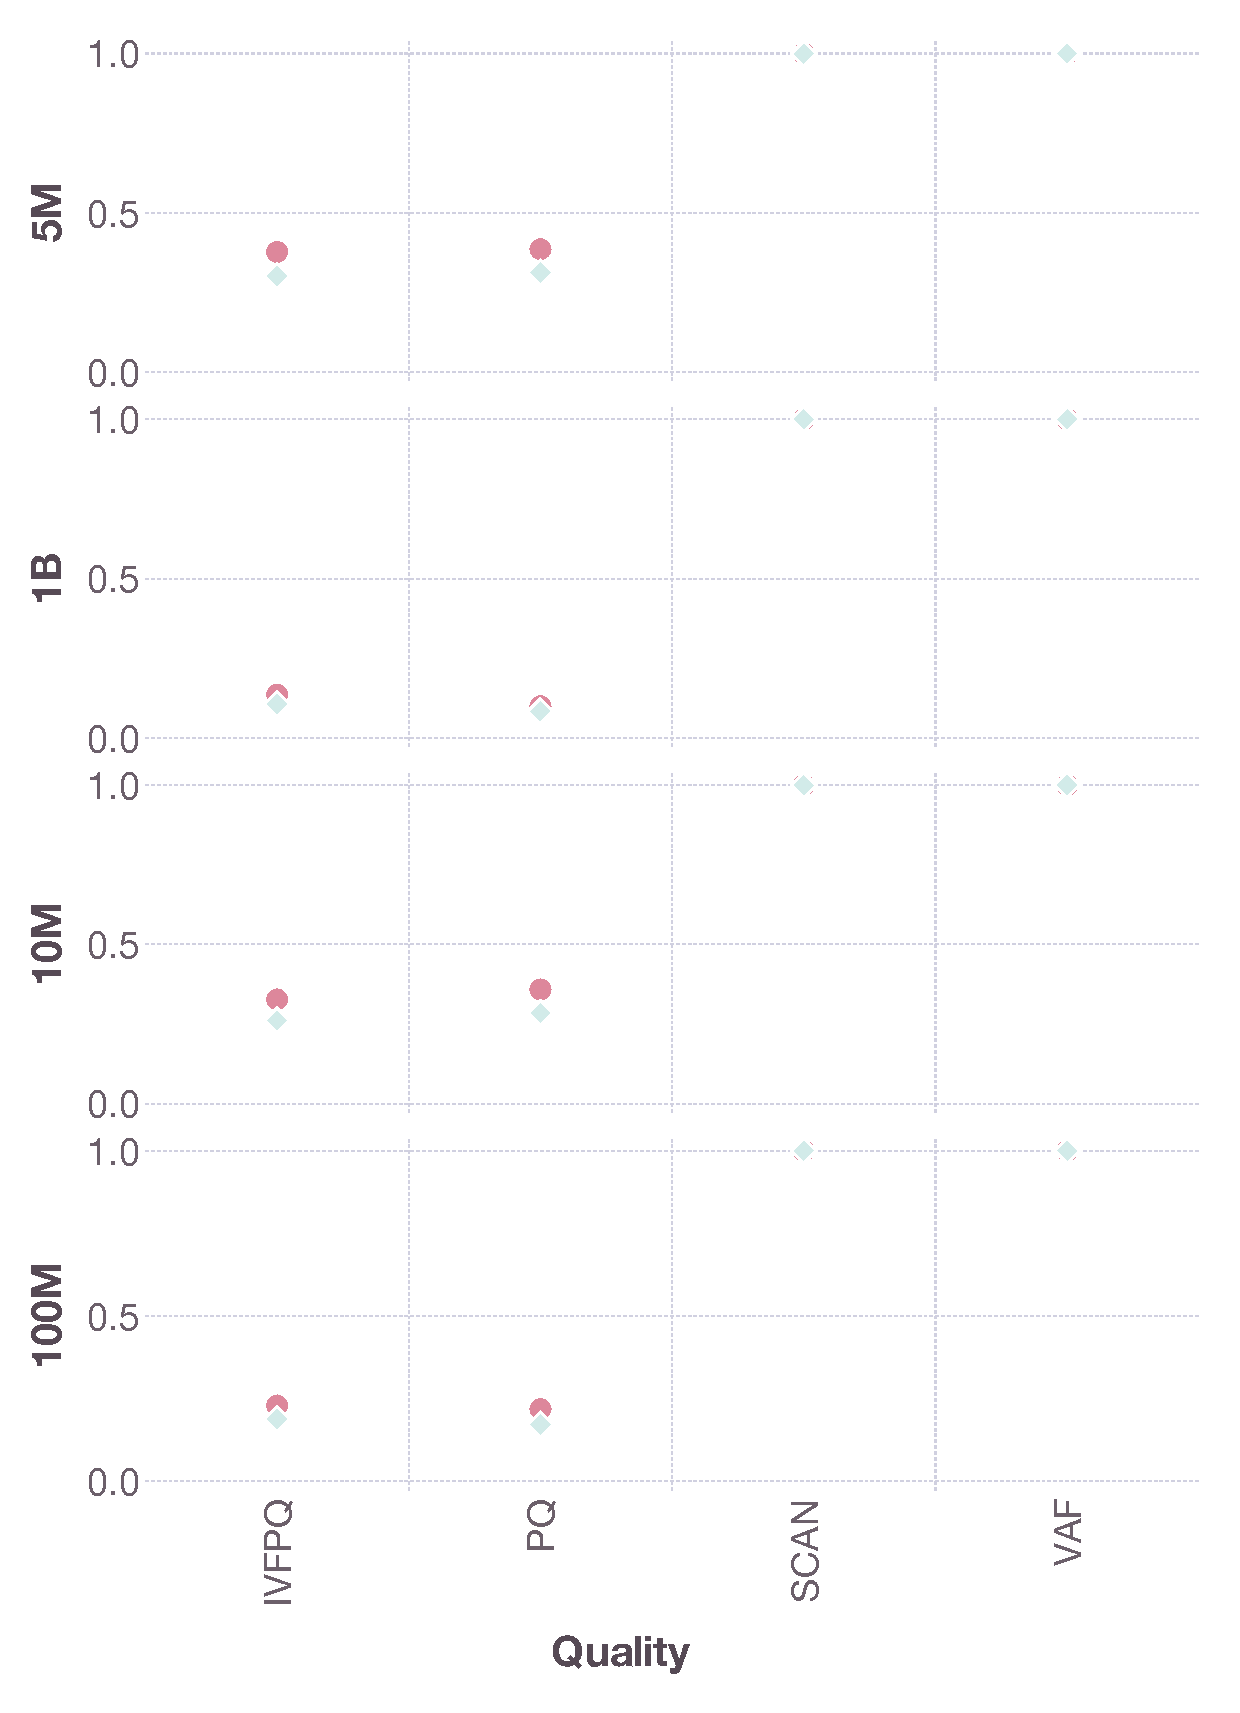
\includegraphics[width=\linewidth]{figures/bignns-cottontail-NNS + Fetch-quality}
    \caption{Quality metrics for Cottontail DB during the \acrshort{nns} + fetch large-scale retrieval evaluation presented in \Cref{section:evaluation_bignns_cottontail}. Recall and \acrshort{dcg} are 1.0 for all execution strategies other than \acrshort{pq}.}
\end{figure}


\begin{figure}[p]
    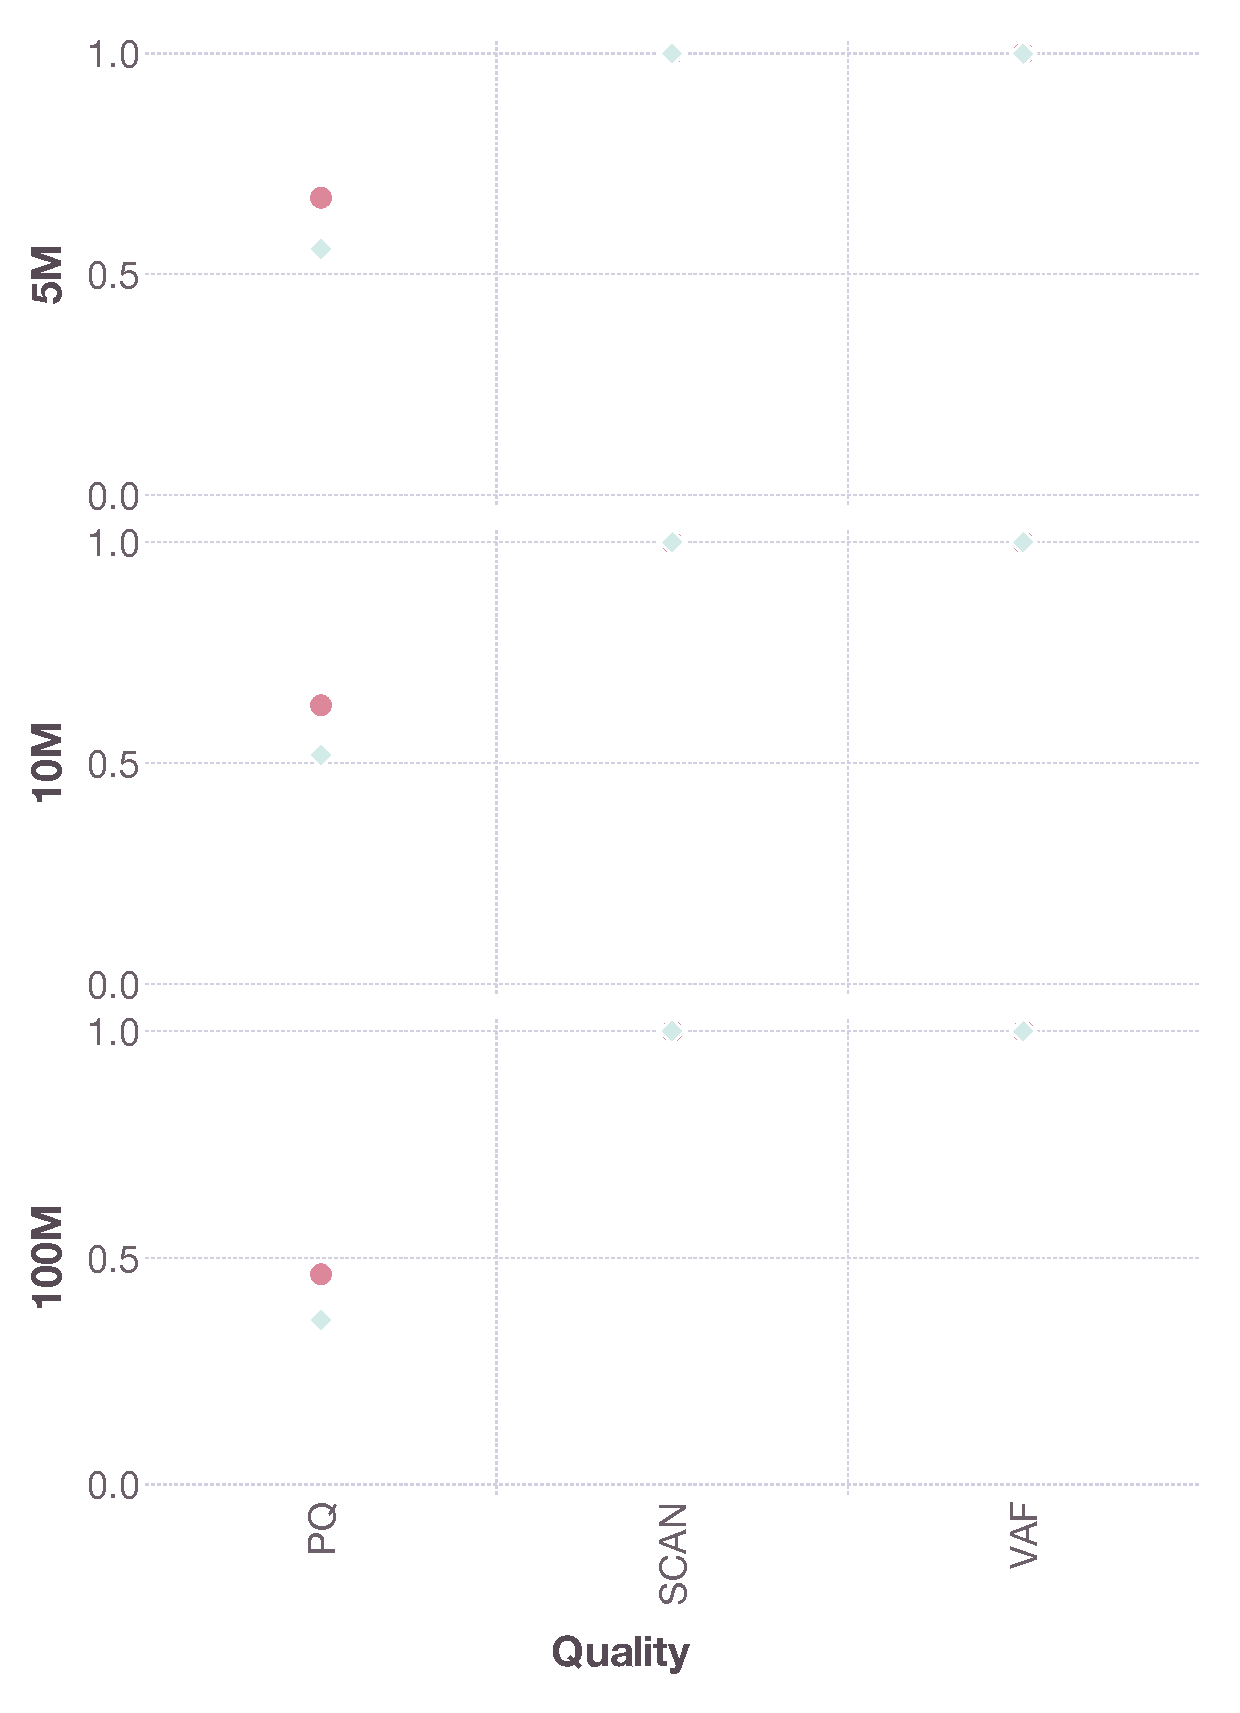
\includegraphics[width=\linewidth]{figures/bignns-cottontail-Hybrid-quality}
    \caption{Quality metrics for Cottontail DB during the hybrid query large-scale retrieval evaluation presented in \Cref{section:evaluation_bignns_cottontail}. Recall and \acrshort{dcg} are 1.0 for all execution strategies other than \acrshort{pq}.}
\end{figure}
